\documentclass[a4paper,10pt]{report}
\usepackage[utf8]{inputenc}
\usepackage{fullpage}
\usepackage{amsmath}
\usepackage{amsfonts}
\usepackage{tikz}
\usepackage{graphicx}
\usepackage{mdframed}
\usepackage{color}
\usepackage{listing}
\usepackage{wrapfig}
\usepackage[parfill]{parskip}
\usepackage{subcaption}
\usepackage{hyperref}
\usepackage[font={small}]{caption}
% Title Page
\title{Facet-based Imaging}
\author{Benjamin Hugo}
\date{April 2014}

\begin{document}
\maketitle
\chapter{Introduction to Radio Astronomy}
In this section we give a very brief overview of what radio astronomy is, how the intensity of celestrial sources are quantified, how these intensity measurements are related to images (synthesis imaging),
the problems faced by large arrays taking measurements over large fields of view, and finally how they can be overcome. The focus of our work lies in acceleration of the synthesis imaging process, and in particular,
focussing on how the current memory intensive techniques required for wide-field imaging can be traded off at the expense of higher computation costs. This tradeoff is qualified by the recent shift towards using 
highly parallel platforms in all major computational fields; ranging in everything from computational chemestry, computing financial models of option pricing, through to radio astronomy. In particular we will be investigating 
the use of General Purpose Graphics Processing Units (GPGPU) in accelerating the facet-based convolutional gridding algorithm. More on this a bit later on.

\section{Brief history}
Through eons of visual observation mankind learned, amongst other things, the laws that govern the movement of the celestrial objects in the skies above him. In the last 500 years we've 
seen major advances in our ability to observe new phenomina, starting with the first optical telescope and manufacture of transparent glass. However these observations
were still restricted to the wavelengths of visible light. Radio waves are about one million times longer than light waves and often exposes areas of space opaque to visible light. The 
next series of improvements exploring this area came only by the 1930s when observations at longer wavelengths were made, after several failed attempts to receive radio emissions from the sun by the 
late nineteenth century. Herschel (1930) expanded the observable electromagnetic spectrum to the near infrared wavelengths: $0.35\mu m \leq\lambda\leq 1\mu m$. The most drastic change came when Jansky (1931) 
observed radiation from an extraterrestrial source (which wasn't the sun) with much longer wavelengths of $14.6m$ using a direction sensitive antenna array. By 1937 Grote Reber published the first observations 
in a professional astronomical journal. After World War II improved equipment and the use of the optical interferometer ultimately lead to the techniques of aperture synthesis still employed today. Ultimately all
historical development has been geared toward shorter wavelengths (see figure~\ref{fig_radio_window}), higher sensitivity, and higher angular resolution\cite{christiansenradiotelescopes,wilson2009tools}.

\begin{figure}[ht]
 \begin{mdframed}
 \centering
 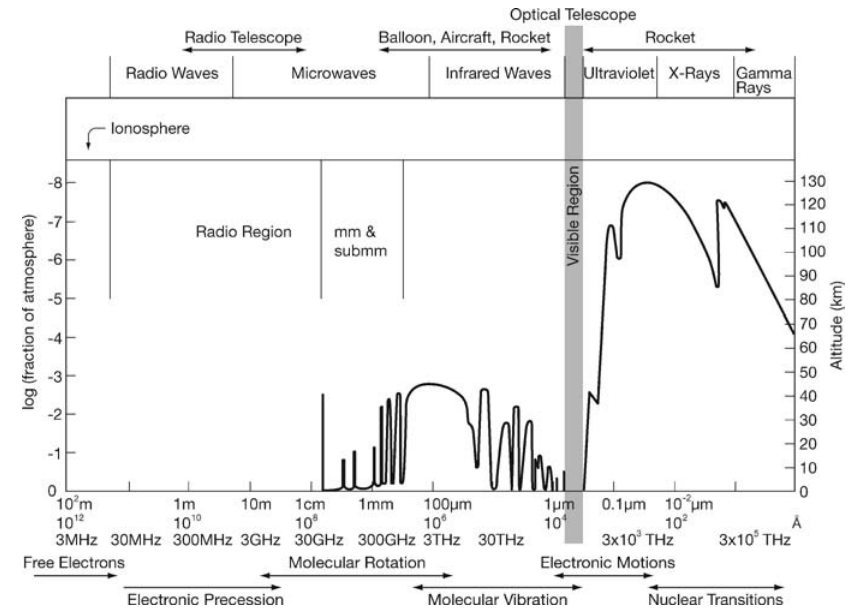
\includegraphics[width=0.8\textwidth]{images/radio_window.png}
 \caption[The radio window]{The radio window - Earth-based radio astronomy is bound to a range of wavelengths between $\lambda\approx 0.2mm$ and $\lambda\approx 20m$ by the molecular absorbtion bands of oxygen and water at the
 small wavelengths and the ionosphere at the long end. The figure shows at what altitude the incomming electromagnetic radiation is attenuated by a factor of 0.5 \cite{wilson2009tools}.}
 \label{fig_radio_window}
 \end{mdframed}
\end{figure}

\section{Review of core signals processing techniques}
Radio astronomy has its roots in Digital Signals Processing. Before diving into the details of how these telescopes work we refer the reader to the \textit{Scientist and Engineer's guide to Digital Signals Processing} by 
Steven Smith\footnote{Available freely at \url{http://www.dspguide.com/}}\cite{smith1997scientist} for a detailed, yet simple overview of the field. A (very) brief overview of some of the core terminology is given here.

A signal is simply a description of how one parameter depends on another. A typical example of this is how voltage varies over time. Since the focus in this thesis lie solely in digitized signals, it is necessary to carefully
define under what circumstances the underlying continuous analog signal can be reconstructed. The Shannon-Nyquest \textit{sampling theorem} forms the cornerstone of Digital Signals Processing. It simply states that the rate at
which samples are taken from a continuous signal has to be at least twice the highest frequency component of that signal. Such a signal is said to be critically sampled if it obeys this minimum requirement. If the requirement is
not satisfied the sampled signal is aliased (higher frequencies appear as low frequency components). This can be illustrated through figure~\ref{fig_invalid_sampling}. Aliasing is usually reduced by applying a filter that essentially
have low responses at frequencies outside a limited \text{passband} of frequencies. This filter is can be something as simple as a windowed sinc function for instance. Although a sharp cutoff frequency is ideal, it should be noted 
that in reality this is not achieved. Filter frequency responces usually decline over a non-infinitesimal section of the spectrum (this is known as \textit{rolloff}).

\begin{figure}[ht]
 \begin{mdframed}
 \centering
 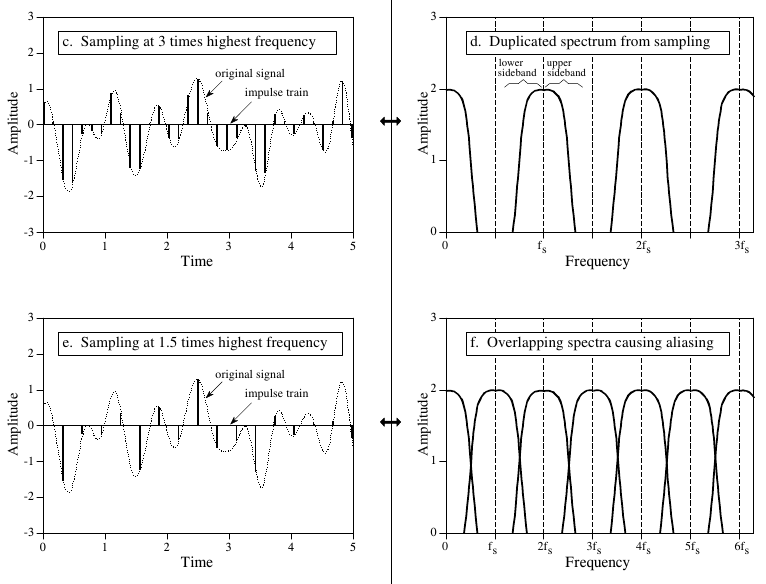
\includegraphics[width=0.8\textwidth]{images/improper_sampling.png}
 \caption[Aliasing]{The first signal is sampled at 3 times the highest composing frequency. Its frequency spectrum shows no overlap between sidebands. The second signal is subsampled and higher frequencies overlap lower frequencies
 in its frequency spectrum. This illustrates a key observation: discarding samples in one domain causes aliasing in the other \cite{smith1997scientist}.}
 \label{fig_invalid_sampling}
 \end{mdframed}
\end{figure}

The next observation is that the propogation of electromagnetic waves and their interactions can be considered as a linear system. This means the signals exhibit three properties: homogeneity, additivity and shift-invariance (the third 
is a non-compulsory property of linearity). We say that the following are true for such systems:

  \begin{flalign*}
    &\textbf{ if }x[n] \rightarrow \text{System} \rightarrow y[n] \textbf{ then } k x[n] \rightarrow \text{System} \rightarrow k y[n] \textit{ (homogeneity)}\\
    &\textbf{ if }x_1[n] \rightarrow \text{System} \rightarrow y_1[n]\textbf{ and }x_2[n] \rightarrow \text{System} \rightarrow y_2[n] \textbf{ then } x_1[n] + x_2[n] \rightarrow \text{System} \rightarrow y_1[n] + y_2[n] \textit{ (additivity)}\\
    &\textbf{ if }x[n] \rightarrow \text{System} \rightarrow y[n] \textbf{ then } x[n + s] \rightarrow \text{System} \rightarrow y[n + s] \textit{ (shift-invariance)}&
  \end{flalign*}

Much of the filtering and imaging techniques described in this thesis rely on the theory of fourier transforms. The fourier transform simply decomposes a continuous periodic signal into a series of sinusoidal terms. A detailed description 
can be found in Smith \cite[ch 8-12,31]{smith1997scientist}, but the general relations between converting between the time and frequency domains (and between the visibility and the intensity spaces as will be described later on) are as follows:
\begin{equation*}
  \begin{split}
    G(f) &= \int_{-\infty}^{\infty}g(x)e^{2\pi ifx}\\
    g(x) &= \int_{-\infty}^{\infty}G(f)e^{-2\pi ifx}
  \end{split}
\end{equation*}
Here capital letters indicate the Fourier space. We will be using this convention throughout this thesis. It is also possible to do this with discrete signals (indicated with square brackets as per convention). In that case the Cooley-Tukey Fast 
Fourier Transform algorithm and its inverse is employed to move between these domains. There are highly optimized libraries available for both C++ (FFTW) and CUDA (cuFFT), and these will be extensively used in our implementations.

For linear systems the following theorems are true (stated without proof):
\begin{equation*}
  \begin{split}
    g_1(x)*g_2(x) &:= \int_{-\infty}^{\infty}g_1(t)g_2(x-t)\textit{ (convolution)}\\
    g_1(x)\star g_2(x) &:= \int_{-\infty}^{\infty}g_1(t)g_2(t+x)\textit{ (cross-correlation)}\\
    &=g_1^*(-x)*g_2(x)\\
    \text{Addition Theorem:}\\
    \mathcal{F}(g_1(x)+g_2(x)) &= G_1(f)+G_2(f)\\
    \text{Convolution Theorem:}\\
    \mathcal{F}(g_1(x)*g_2(x)) &=G_1(f).G_2(f)\\
    \mathcal{F}(g_1(x).g_2(x)) &=G_1(f)*G_2(f)\\
    \text{Shift Theorem:}\\
    \mathcal{F}(g(x-\Delta))&=G(f)e^{-2\pi if\Delta}
  \end{split}
\end{equation*}

In general the convolution is known as filtering, the cross-correlation can be seen as ``time averaging between two signals'' and signal shifting essentially shifts the directional cosine (as seen in the next section) and electrically
stears the telescope. The two dimensional versions of convolution, cross-correlation, the fourier transform and its inverse are analoguous to their one dimensional counterparts. The two dimensional fourier transform first transforms
over one axis and then transforms the output on the second axis. Two-dimensional convolution is similar provided the filter is seperable, meaning $h[m,n]=h_1[m]h_2[n]$. This last statement provides a significant speed improvement. More 
on this later on.
\section{Measuring flux with a single element telescope}
Some of the most important measurements of a celestrial object includes the object's angular size, position (according to some celestrial coordinate system) and the \textit{flux} density over a 
frequency spectrum of the object. The flux density is measured as the power per square meter per unit frequency, falling on a surface, normal to the direction of the source. This flux 
density of sources is often a very small value and the Jansky (abbreviated Jy) serves as the unit of measure \cite{christiansenradiotelescopes,wilson2009tools}:

\begin{equation*}
 1 Jy := 10^{-26}Wm^{-2}Hz^{-1}
\end{equation*}

Electromagnetic radiation is a wave phenominon stemming from both thermal and non-thermal sources propagating outward at the speed of light. Generally thermal sources follows Rayleigh's approximation to the radiation 
law and states that a black-body will have a flux density $S\propto \upsilon^2T$ where the black-body radiates at a temperature $T^oK$. The spectra of planets and stars are of this type. On the other hand in non-thermal 
sources, one of the most common generators of electromagnetic ratiation magnetic is \textit{synchrotron emission}. This process accelerates the electrons passing through electric fields. A significant portion of radio 
astronomy focusses on the non-thermal sources. These are generally very intense sources of electromagnetic radiation and are very far away \cite{christiansenradiotelescopes}.

It is worth noting that not only are radio telescopes used to observe continuous spectra consisting of a wide band of frequencies, but it is also critical sometimes to isolate a number of
spectral lines for observation. These don't originate from large black-body structures, but focusses on the detection of certain molecules, such as neutral hydrogen (at $\lambda = 21 cm$) and
hydroxyl ($\lambda \approx 18 cm)$. These spectral lines are vital in measuring radial velocities through Doppler frequency shift \cite{christiansenradiotelescopes}.

It should be clear that since most sources are extremely faint, the telescopes needed to detect them will be some of the most sensitive instruments ever designed. Although we cannot
cover antenna theory extensively here, it is essential to briefly relate how the electromagnetic radiation covered earlier, is measured by instrumentation in general, as well as some of the constraints under which
these measurements are made.

The wave fronts from distant sources can be viewed as planar fronts if the source of the radiation is sufficiently far away. This is not necessarily true for sources within our own galaxy for example. Furthermore 
if the wavelength is much smaller than the scale of the phenomena the radiation can be viewed as rays. In radio astronomy these measures serve only as rough discriptions of the 
equations that govern wave propagation, as the wavelengths are significantly longer than in optical systems.  The total flux of a source is then obtained over the solid angle subtended by the 
source (see figure~\ref{fig_measuring_source_brightness}) as follows \cite{wilson2009tools}:

  \begin{equation}
    S_v := \int_{\Omega_s}{I_v(\theta,\phi)\cos{\theta}d\Omega}
  \end{equation}
  and the infinitesimal power intercepted by an infinitesimal surface is:
  \begin{equation}
    dP = I_v\cos{\theta}d\Omega\ d\sigma d\upsilon
  \end{equation}

  where:\\
  $dP = $ infinitesimal power (in watts)\\
  $d\sigma = $ infintesimal area of surface\\
  $d\upsilon = $ infintesimal bandwidth\\
  $\theta = $ angle between the direction to $d\Omega$ and normal to the surface\\
  $I_{v} =$ specific intensity in $Wm^{-2}Hz^{-1}sr^{-1}$ where r is the distance between the source and antenna.\\
  
\begin{figure}[ht]
\begin{mdframed}
 \centering
 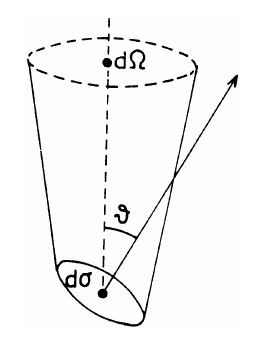
\includegraphics[width=0.2\textwidth]{images/measuring_source_brightness.png}
 \caption[Source brightness]{Flux density over a small area per unit frequency \cite{wilson2009tools}.}
 \label{fig_measuring_source_brightness}
\end{mdframed}
\end{figure}

For the sake of simplicity we will only consider a single simple parabollic reflector telescope for now to explain the general concepts of the primary beam and what impact it has on wide-field observations. Synthesis imaging \cite[ch. 3]{taylor1999synthesis} 
gives a more extensive overview of different antennae optics and mountings. Filled reflector antennas are normally used for $\lambda \geq 1m$, whereas unfilled ``wire'' antennae are frequently used at shorter wavelengths. We can describe
the operation of these parabollic reflectors using Huygen's principle \cite{christiansenradiotelescopes}: 
\begin{quote}
The energy at the focus of the telescope is the sum of the of the contributions from all parts of the incoming wave-front, taking into account the different path lengths and therefore different radio-frequency phases at the focus.
\end{quote}
The power available for a feed antenna placed at the focal point is proportional to the square intensity of the field of view and is known as the beam of the antenna and varies with the angle of incidence betweeen the the waves and the pointing of
direction of the antenna, see figure~\ref{diffraction_pattern_and_power_at_focus}. It should therefore be clear the telescope has a limited effective area of view. It turns out that the size of the aperture of the telescope plays a key role
in the resolving power of the telescope, which is limited by the diffraction patterns as seen in figure~\ref{diffraction_pattern_and_power_at_focus}. Any object larger than the primary beam of the antennae will be aliased to a certain
extent by the sidelobes shown in figure~\ref{diffraction_pattern_and_power_at_focus}, although the general structure may still be the same:
\begin{equation*}
 \text{resolving power} \propto \frac{\lambda}{D}
\end{equation*}
\begin{figure}[ht]
 \begin{mdframed}
  \centering
  \begin{subfigure}[b]{0.3\textwidth}
   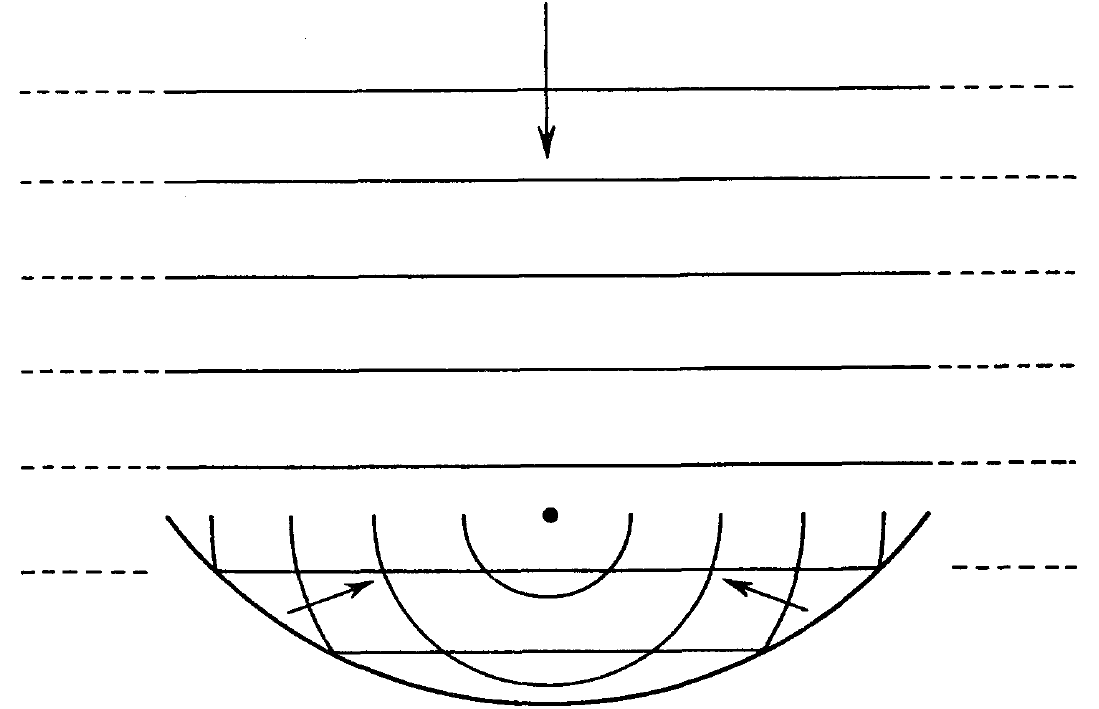
\includegraphics[width=\textwidth]{images/diffraction_pattern.png}
   \caption{}
  \end{subfigure}
  \begin{subfigure}[b]{0.3\textwidth}
   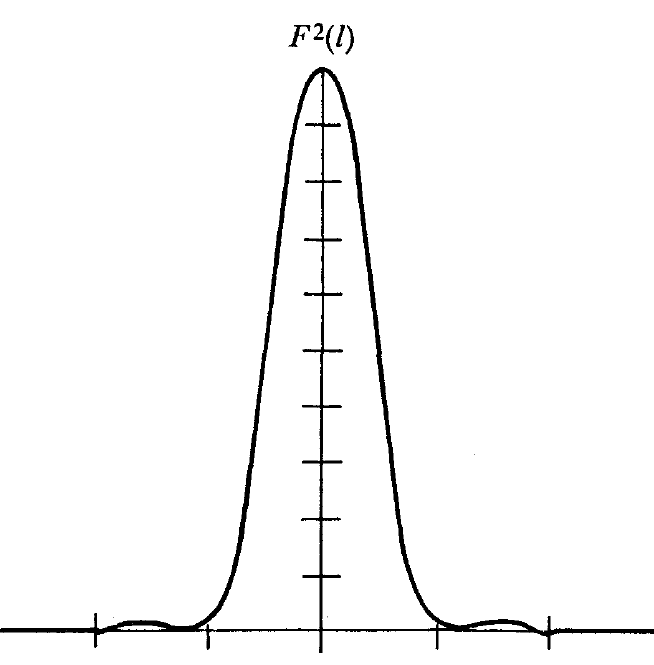
\includegraphics[width=\textwidth]{images/field_strength_in_the_focal_plane.png}
   \caption{}
  \end{subfigure}
  \begin{subfigure}[b]{0.3\textwidth}
   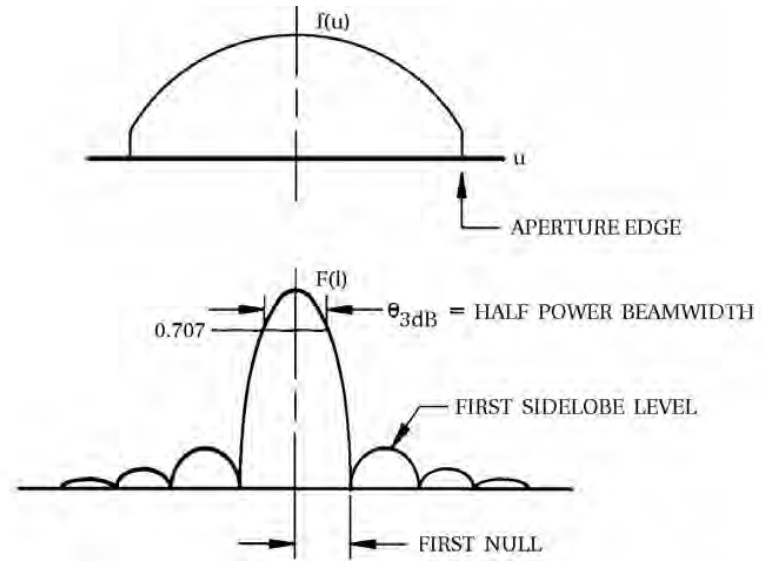
\includegraphics[width=\textwidth]{images/radiation_pattern.png}
   \caption{}
  \end{subfigure}
  \caption[Collection of electromagnetic wave energy and responce]{In (a) we illustrate the defraction pattern of a parabollic aperture and how the total energy is collected at the focal point \cite{christiansenradiotelescopes}. In (b) the power at the antenna terminals
  is significantly higher for small angles from the antenna pointing direction \cite{christiansenradiotelescopes}. Lastly in (c) we give a 1 dimensional illustration of the effects of apperture form and diameter on the antenna's effective resolving capability. If objects
  larger than the center beam is observed the objects will be effectively aliased by the ``sidelobes'' off both ends of the ``primary'' beam. The response is the \textit{fourier transform} of the shape of the aperture. It should now be clear
  that the effective collection area, $A(l,m)$ approaches the geometric area of the apperture in the direction of maximum response \cite{taylor1999synthesis}.}
  \label{diffraction_pattern_and_power_at_focus}
 \end{mdframed}
\end{figure}

Another key observation to take into consideration are the effects of polarization in electomagnetic wavefronts. All electromagnetic radiation can be characterised by a field vector parallel to to the wavefront. This wavefront is said to
be either elliptically polarized if the field vector traces out an ellipse of constant orientation and eccentricity (linear and circular polirization are special cases of this). On the other hand it may be randomly polarized (or ``unpolarized'') if the field 
vector changes randomly. To capture the total energy of of the electromagnetic field any antenna should have two independent feeds to resolve any radio wave, where the second feed must be placed at right angles to the first. The first and second feeds will carry, 
on average equal amounts of power. The total flux density is therefore the sum of both polarized feeds \cite{christiansenradiotelescopes}.

Up to this point we've assumed that the energy measured at the focus point of the telescope is attributed to a single point source. In reality many sources contribute to the specific intensity integral over the solid angle $d\Omega$. These point sources
are generally accepted to be completely uncorrelated, and therefore the mean squared voltage at each of the antenna feeds is a linear combination from each of these sources (weighted by the effective area function $A(l,m)$) \cite{christiansenradiotelescopes}. In general this requires instrument 
calibration to be done over all the bright sources in the beam-limited field of view. More on calibration techniques later on.

\section{Interferometric telescopes}
As pointed out in the previous section the angular resolution is constrained to the diameter of the telescope. Unfortunately there are material constraints to the size of an apperture ($\sim 300m$ as pointed out in \cite{wilson2009tools}). The Arecibo Observatory, Puerto Rico is the extreme case 
of this, see fig~\ref{fig_arecibo}. Luckily the same resolving power may also be obtained by \textit{coherently} combining the feeds from two reflectors, seperated by a straight-line distance, $B$:
\begin{equation*}
 \text{resolving power} \propto \frac{\lambda}{B} \text{ if } D\ll B
\end{equation*}
\begin{figure}[ht]
 \begin{mdframed}
 \centering
 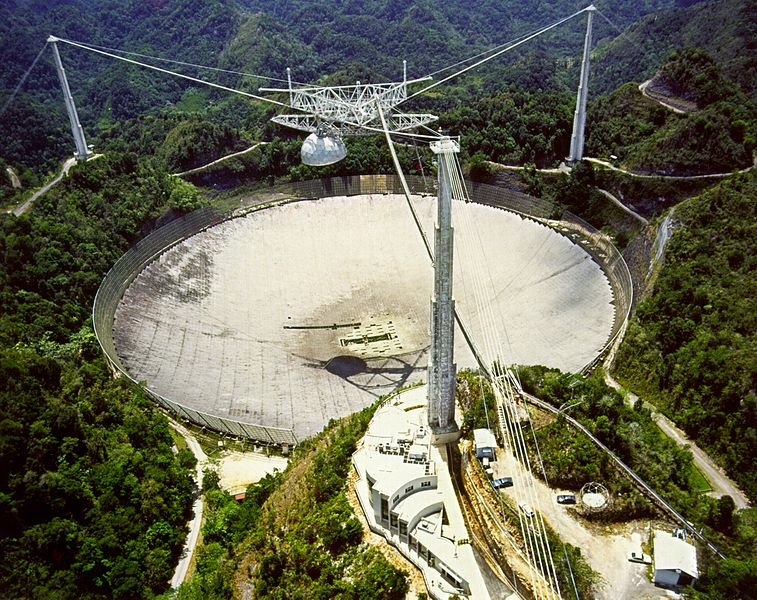
\includegraphics[width=0.7\textwidth]{images/arecibo.jpg}
 \caption[Arecibo Observatory]{At a wopping 305m diameter, the telescope at the Arecibo Observatory is the largest single-apperature telescope in the world. Image courtesy of the National Oceanic and Atmospheric Administration (public domain).}
  \label{fig_arecibo}
 \end{mdframed}
\end{figure}
This combination process synthesizes a larger aperture (in general this aperture is unfilled \cite{christiansenradiotelescopes}), with the first practical demonstration made by Ryle and his associates. The feeds from two antennae are joined by a 
correlator which, can be thought of, as taking short-time averages. When the antennae are spaced $B$ units appart the electromagnetic wavefront will reach one telescope before reaching the other (figure~\ref{fig_cosine_correlator}). This delay, 
$\tau=\frac{\vec{b}\cdot\vec{s}}{c}$ is usually compensated for by the correlator in order to achieve a coherent correlation (as mentioned previously). For short intervals the correlator response (for a planar wavefront) over all the sources in 
the effective collection area is (refer to figure~\ref{fig_cosine_correlator}) \cite{taylor1999synthesis}:
\begin{equation}
\label{eqn_cosine_correlation}
r=\Delta\upsilon \int_{\vec{s}}{A(\vec{s})I(\vec{s})\cos{\frac{2\pi\vec{b}\cdot\vec{\sigma}}{\lambda}}d\Omega}
\end{equation}

\begin{figure}[ht]
 \begin{mdframed}
 \centering
 \begin{subfigure}[b]{0.3\textwidth}
 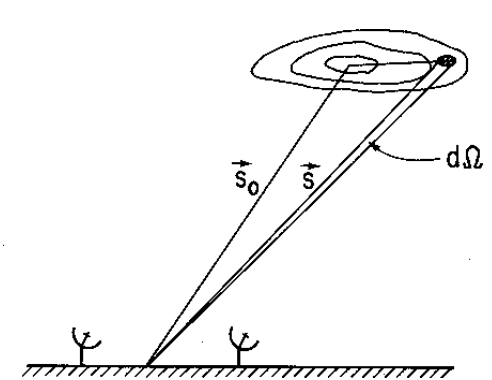
\includegraphics[width=\textwidth]{images/phase_center.png}
 \caption{}
 \end{subfigure}
 \begin{subfigure}[b]{0.4\textwidth}
 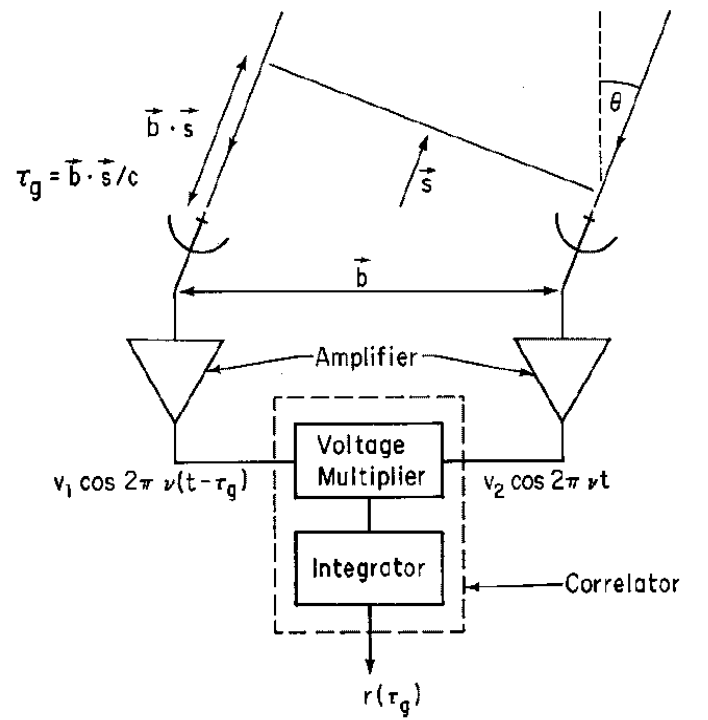
\includegraphics[width=\textwidth]{images/cosine_correlator.png}
 \caption{}
 \end{subfigure}
 \begin{subfigure}[b]{0.2\textwidth}
 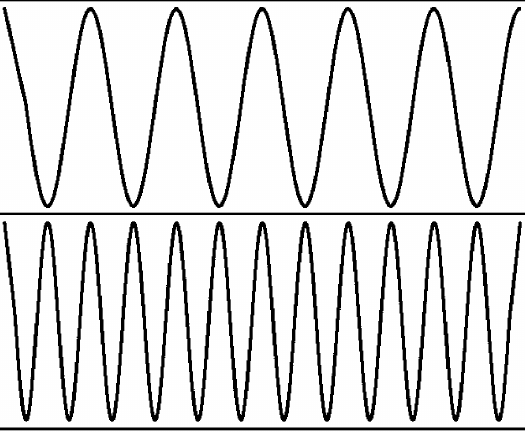
\includegraphics[width=\textwidth]{images/fringe.png}
 \caption{}
 \end{subfigure}
 \caption[Cosine correlator]{(a) Position vectors used in the interferometer response. $\vec{s_0}$ is the \textit{phase tracking center} where $\tau:=0$ \cite{taylor1999synthesis} (b) Simplified diagram of a two-element correlator, combining the output of two elements spaced $B=||\vec{b}||$ appart. The integrator takes the \textit{cross correlation} of the signal 
 from the second telescope and a time-delayed signal from the first telescope over a small period of time \cite{taylor1999synthesis}. (c) The power produced through cross correlation, differs from that of a single element telescope as shown in figure~\ref{diffraction_pattern_and_power_at_focus} and has a response for greater angles than a small single reflector telescope. If $B$ is doubled, 
 the fringe width is halved and the the correlator response for larger angles improves. \cite{wilson2009tools}.}
  \label{fig_cosine_correlator}
 \end{mdframed}
\end{figure}
It is easy to see that this correlator ``fringe'' pattern has a major drawback: the correlator is insensitive for $\frac{2\pi\vec{b}\cdot\vec{\sigma}}{\lambda} = \frac{\pi}{2} \pm n\pi$. To fix this problem correlators typically
take the form of \textit{complex correlators} where a second correlation is made by introducing a phase delay of $\frac{\pi}{2}$ in the feeds of the antennae. The second correlator is effectively a \textit{sine correlator}. We can
now replace the cosine term in equation~\ref{eqn_cosine_correlation} by $e^{-2\pi\vec{b}\cdot\vec{\sigma}/\lambda}$ through the Euler relation between the complex exponential and the polar form of a complex coordinate \cite{taylor1999synthesis}.

The next issue are the effects of limited \textit{bandwidth}, $\Delta\upsilon$, in correlators. Since it is computationally infeasible to sample an infinite spectrum of frequencies, only a select number of channels are sampled. This
band is normally shifted down to \textit{baseband} ($\upsilon=0$) and filtered appropriately with a lowpass filter to reduce aliasing, refer to figure~\ref{fig_bandwidth}. The baseline is normally measured in wavelengths and therefore depends on the
center frequency through the well-known relation $\upsilon=\frac{c}{\lambda}$. Unfortunately this has a negative impact on the fringe pattern of the correlator; the fringe is modulated by a sinc-function for a rectangular band. This has
the effect of tapering the fringe which again reduces the effective area of the interferometric telescope. The obvious solution is to observe only narrow spectra. The fringe depends on the delay term and oscilates in time. Normally this is not a problem.
However, with exceedingly long baselines such as those in \textit{Very Long Baseline Interferometry}, where the baselines may span continents (see Middelberg et al. \cite{middelberg2008high} for a detailed overview), the local oscilator term is usually varied 
by a delay tracking computer, which essentially stops any fringe oscilation (known as \textit{fringe stopping}) \cite{taylor1999synthesis}.
\begin{figure}
 \begin{mdframed}
 \centering
 \begin{subfigure}[b]{0.3\textwidth}
 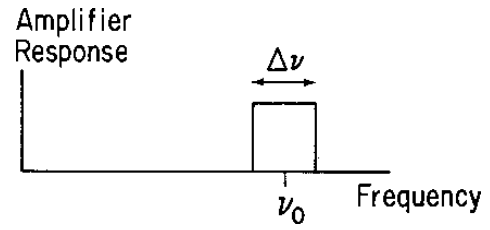
\includegraphics[width=\textwidth]{images/rectangular_band.png}
 \caption{}
 \end{subfigure}
 \begin{subfigure}[b]{0.5\textwidth}
 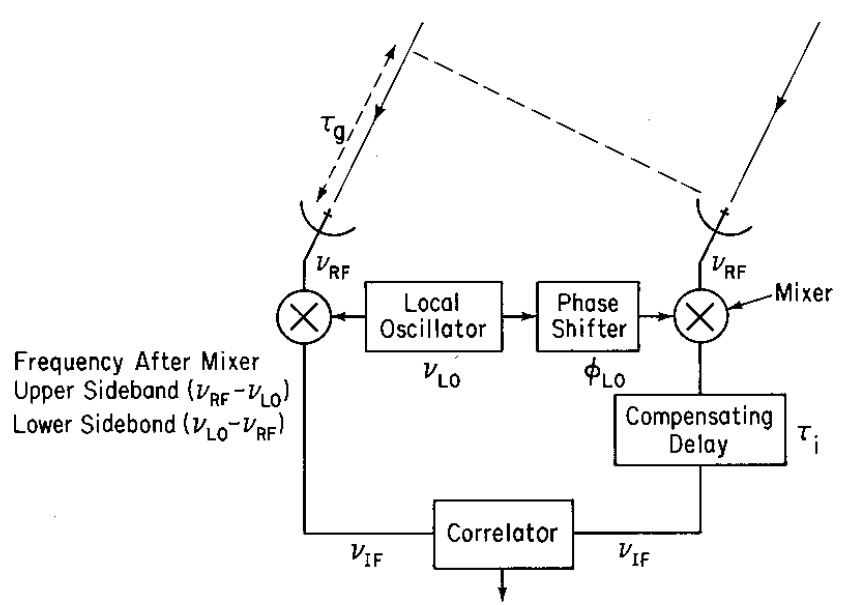
\includegraphics[width=\textwidth]{images/mixing.png}
 \caption{}
 \end{subfigure}
 \caption[Sampling a limited bandwidth]{(a) illustrates the idealized rectangular responce of the correlator. Due to inevitable filter rolloff this is obviously unatainable \cite{taylor1999synthesis}. (b) For practical
 reasons the signal is shifted to baseband before filtering out higher frequencies. This is achieved by multiplying the signal with a tone produced by a local oscilator (mixing) this shifts the 
 frequency response of the correlator by $\pm\upsilon_{lo}$ \cite{taylor1999synthesis}} 
  \label{fig_bandwidth}
 \end{mdframed}
\end{figure}

Up to this point we conveniently only discussed correlator output for a single feed of each antenna in a two element interferometer. The correlator additionally cross-correlates the two polarization feeds to form the following matrix of complex cross-correlations between the
antennae p \& q (where * indicates the complex conjugate). The equation governing the correlator power response remain the same. Here I, V, U and Q are the four Stokes parameters \cite{taylor1999synthesis}.
\begin{equation}
X_{pq} = \left[\begin{array}{c c}
     e_{X_pX_q^*} & e_{X_pY_q^*} \\
     e_{Y_pX_q^*} & e_{Y_pY_q^*} \\
    \end{array}\right] = 
    \left[\begin{array}{c c}
     I + V & Q + iU \\
     Q - iU & I - V \\
    \end{array}\right]
\end{equation}
Each of the parameters Q, U and V are linearly independent and discribe a position on the Poincar\'e Sphere (figure \ref{fig_poincare}). Their coordinates on the sphere are given by
\begin{equation}
  \begin{split}
    Q &= I\cos{2\chi}\cos{2\psi}\\
    U &= I\cos{2\chi}\sin{2\psi}\\
    V &= I\sin{2\chi}\\
  \end{split}
\end{equation}

\begin{figure}
 \begin{mdframed}
 \centering
 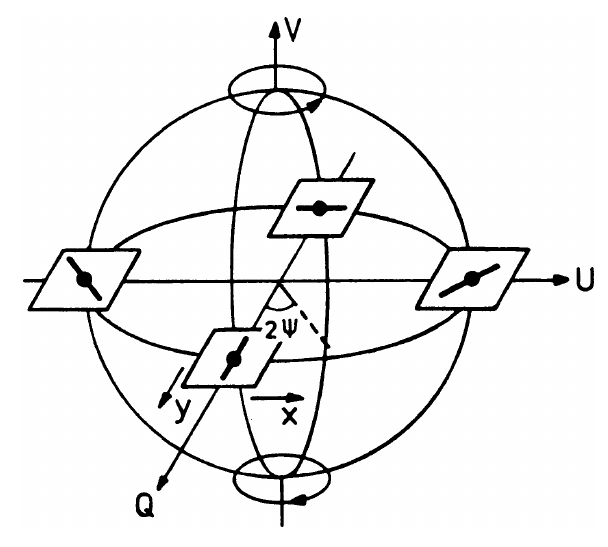
\includegraphics[width=0.45\textwidth]{images/poincare_sphere.png}
 \caption[The Poincar\'e Sphere]{The Poincar\'e Sphere gives a visualization for the different polarizations an electromagnetic field. The angles $2\psi$ and
 $2\chi$ are the angles in a polar coordinate system, with each point on the sphere corresponding to a unique polarization. At $2\chi=0$ (the equator) the polarizations 
 are either linear (Q) and orthagonal (U). The northern latitudes ($2\chi > 0$) contain right-handed circular polarization, while the southern hemisphere 
 contains the left-handed circular polarizations. $I$ is not linearly independent and describes the total Poynting flux of the electromagnetic wave; $I = E_1^2 + E_2^2$ \cite{wilson2009tools}}
  \label{fig_poincare}
 \end{mdframed}
\end{figure}

It is worthwhile to note that the correlation, delay and phase compensations can also be done in the fourier domain, and in the case of delay compensation this approach makes fractional delay compensation feasible (see Taylor et al. \cite{taylor1999synthesis}). These correlators are effectively 
known as \textit{FX} correlators. If these power spectra are of high time resolution it is possible to perform surveys focussed on transient detection. Modern arrays such as LOFAR, KAT-7 and MeerKAT (currently under construction) have the capability to perform these searches through
special \textit{beamforming} modes which may be run concurrently with imaging modes. See Stappers et al. \cite{stappers2011observing} for details on pulsar observation with LOFAR. In this thesis, however, we will focus solely on the imaging pipeline which is discussed in the next section.

\section{Synthesis imaging}
{\color{red} TODO}

\bibliography{bibfile}
\bibliographystyle{plain}
\end{document}          
